% Options for packages loaded elsewhere
% Options for packages loaded elsewhere
\PassOptionsToPackage{unicode}{hyperref}
\PassOptionsToPackage{hyphens}{url}
%
\documentclass[
  11pt,
  ignorenonframetext,
  aspectratio=169,
]{beamer}
\newif\ifbibliography
\usepackage{pgfpages}
\setbeamertemplate{caption}[numbered]
\setbeamertemplate{caption label separator}{: }
\setbeamercolor{caption name}{fg=normal text.fg}
\beamertemplatenavigationsymbolsempty
% remove section numbering
\setbeamertemplate{part page}{
  \centering
  \begin{beamercolorbox}[sep=16pt,center]{part title}
    \usebeamerfont{part title}\insertpart\par
  \end{beamercolorbox}
}
\setbeamertemplate{section page}{
  \centering
  \begin{beamercolorbox}[sep=12pt,center]{section title}
    \usebeamerfont{section title}\insertsection\par
  \end{beamercolorbox}
}
\setbeamertemplate{subsection page}{
  \centering
  \begin{beamercolorbox}[sep=8pt,center]{subsection title}
    \usebeamerfont{subsection title}\insertsubsection\par
  \end{beamercolorbox}
}
% Prevent slide breaks in the middle of a paragraph
\widowpenalties 1 10000
\raggedbottom
\AtBeginPart{
  \frame{\partpage}
}
\AtBeginSection{
  \ifbibliography
  \else
    \frame{\sectionpage}
  \fi
}
\AtBeginSubsection{
  \frame{\subsectionpage}
}
\usepackage{iftex}
\ifPDFTeX
  \usepackage[T1]{fontenc}
  \usepackage[utf8]{inputenc}
  \usepackage{textcomp} % provide euro and other symbols
\else % if luatex or xetex
  \usepackage{unicode-math} % this also loads fontspec
  \defaultfontfeatures{Scale=MatchLowercase}
  \defaultfontfeatures[\rmfamily]{Ligatures=TeX,Scale=1}
\fi
\usepackage{lmodern}

\ifPDFTeX\else
  % xetex/luatex font selection
\fi
% Use upquote if available, for straight quotes in verbatim environments
\IfFileExists{upquote.sty}{\usepackage{upquote}}{}
\IfFileExists{microtype.sty}{% use microtype if available
  \usepackage[]{microtype}
  \UseMicrotypeSet[protrusion]{basicmath} % disable protrusion for tt fonts
}{}
\makeatletter
\@ifundefined{KOMAClassName}{% if non-KOMA class
  \IfFileExists{parskip.sty}{%
    \usepackage{parskip}
  }{% else
    \setlength{\parindent}{0pt}
    \setlength{\parskip}{6pt plus 2pt minus 1pt}}
}{% if KOMA class
  \KOMAoptions{parskip=half}}
\makeatother

\usepackage{color}
\usepackage{fancyvrb}
\newcommand{\VerbBar}{|}
\newcommand{\VERB}{\Verb[commandchars=\\\{\}]}
\DefineVerbatimEnvironment{Highlighting}{Verbatim}{commandchars=\\\{\}}
% Add ',fontsize=\small' for more characters per line
\usepackage{framed}
\definecolor{shadecolor}{RGB}{241,243,245}
\newenvironment{Shaded}{\begin{snugshade}}{\end{snugshade}}
\newcommand{\AlertTok}[1]{\textcolor[rgb]{0.68,0.00,0.00}{#1}}
\newcommand{\AnnotationTok}[1]{\textcolor[rgb]{0.37,0.37,0.37}{#1}}
\newcommand{\AttributeTok}[1]{\textcolor[rgb]{0.40,0.45,0.13}{#1}}
\newcommand{\BaseNTok}[1]{\textcolor[rgb]{0.68,0.00,0.00}{#1}}
\newcommand{\BuiltInTok}[1]{\textcolor[rgb]{0.00,0.23,0.31}{#1}}
\newcommand{\CharTok}[1]{\textcolor[rgb]{0.13,0.47,0.30}{#1}}
\newcommand{\CommentTok}[1]{\textcolor[rgb]{0.37,0.37,0.37}{#1}}
\newcommand{\CommentVarTok}[1]{\textcolor[rgb]{0.37,0.37,0.37}{\textit{#1}}}
\newcommand{\ConstantTok}[1]{\textcolor[rgb]{0.56,0.35,0.01}{#1}}
\newcommand{\ControlFlowTok}[1]{\textcolor[rgb]{0.00,0.23,0.31}{\textbf{#1}}}
\newcommand{\DataTypeTok}[1]{\textcolor[rgb]{0.68,0.00,0.00}{#1}}
\newcommand{\DecValTok}[1]{\textcolor[rgb]{0.68,0.00,0.00}{#1}}
\newcommand{\DocumentationTok}[1]{\textcolor[rgb]{0.37,0.37,0.37}{\textit{#1}}}
\newcommand{\ErrorTok}[1]{\textcolor[rgb]{0.68,0.00,0.00}{#1}}
\newcommand{\ExtensionTok}[1]{\textcolor[rgb]{0.00,0.23,0.31}{#1}}
\newcommand{\FloatTok}[1]{\textcolor[rgb]{0.68,0.00,0.00}{#1}}
\newcommand{\FunctionTok}[1]{\textcolor[rgb]{0.28,0.35,0.67}{#1}}
\newcommand{\ImportTok}[1]{\textcolor[rgb]{0.00,0.46,0.62}{#1}}
\newcommand{\InformationTok}[1]{\textcolor[rgb]{0.37,0.37,0.37}{#1}}
\newcommand{\KeywordTok}[1]{\textcolor[rgb]{0.00,0.23,0.31}{\textbf{#1}}}
\newcommand{\NormalTok}[1]{\textcolor[rgb]{0.00,0.23,0.31}{#1}}
\newcommand{\OperatorTok}[1]{\textcolor[rgb]{0.37,0.37,0.37}{#1}}
\newcommand{\OtherTok}[1]{\textcolor[rgb]{0.00,0.23,0.31}{#1}}
\newcommand{\PreprocessorTok}[1]{\textcolor[rgb]{0.68,0.00,0.00}{#1}}
\newcommand{\RegionMarkerTok}[1]{\textcolor[rgb]{0.00,0.23,0.31}{#1}}
\newcommand{\SpecialCharTok}[1]{\textcolor[rgb]{0.37,0.37,0.37}{#1}}
\newcommand{\SpecialStringTok}[1]{\textcolor[rgb]{0.13,0.47,0.30}{#1}}
\newcommand{\StringTok}[1]{\textcolor[rgb]{0.13,0.47,0.30}{#1}}
\newcommand{\VariableTok}[1]{\textcolor[rgb]{0.07,0.07,0.07}{#1}}
\newcommand{\VerbatimStringTok}[1]{\textcolor[rgb]{0.13,0.47,0.30}{#1}}
\newcommand{\WarningTok}[1]{\textcolor[rgb]{0.37,0.37,0.37}{\textit{#1}}}

\usepackage{longtable,booktabs,array}
\newcounter{none} % for unnumbered tables
\usepackage{calc} % for calculating minipage widths
\usepackage{caption}
% Make caption package work with longtable
\makeatletter
\def\fnum@table{\tablename~\thetable}
\makeatother
\usepackage{graphicx}
\makeatletter
\newsavebox\pandoc@box
\newcommand*\pandocbounded[1]{% scales image to fit in text height/width
  \sbox\pandoc@box{#1}%
  \Gscale@div\@tempa{\textheight}{\dimexpr\ht\pandoc@box+\dp\pandoc@box\relax}%
  \Gscale@div\@tempb{\linewidth}{\wd\pandoc@box}%
  \ifdim\@tempb\p@<\@tempa\p@\let\@tempa\@tempb\fi% select the smaller of both
  \ifdim\@tempa\p@<\p@\scalebox{\@tempa}{\usebox\pandoc@box}%
  \else\usebox{\pandoc@box}%
  \fi%
}
% Set default figure placement to htbp
\def\fps@figure{htbp}
\makeatother





\setlength{\emergencystretch}{3em} % prevent overfull lines

\providecommand{\tightlist}{%
  \setlength{\itemsep}{0pt}\setlength{\parskip}{0pt}}



 


\setbeamertemplate{navigation symbols}{}
\setbeamertemplate{footline}[frame number]
\setbeamertemplate{itemize items}[circle]
\setbeamertemplate{itemize subitem}[triangle]
\setbeamercolor{frametitle}{fg=black}
\setbeamerfont{frametitle}{series=\bfseries}
\newcommand{\indep}{\perp\!\!\!\perp}
\usepackage{booktabs}
\usepackage{tikz}
\usetikzlibrary{arrows.meta,positioning,calc}
\tikzset{
  dnode/.style={circle,draw,thick,minimum size=9mm,inner sep=1pt,font=\small},
  unode/.style={circle,draw,thick,dashed,minimum size=9mm,inner sep=1pt,font=\small},
  qnode/.style={circle,draw,thick,dotted,minimum size=9mm,inner sep=1pt,font=\small},
  de/.style={-{Stealth[length=2.2mm]},thick},
  dde/.style={-{Stealth[length=2.2mm]},thick,dashed}
}
\usepackage{fancyvrb}
\fvset{fontsize=\scriptsize}
\makeatletter
\def\verbatim@font{\scriptsize\ttfamily}
\makeatother
\makeatletter
\@ifpackageloaded{caption}{}{\usepackage{caption}}
\AtBeginDocument{%
\ifdefined\contentsname
  \renewcommand*\contentsname{Table of contents}
\else
  \newcommand\contentsname{Table of contents}
\fi
\ifdefined\listfigurename
  \renewcommand*\listfigurename{List of Figures}
\else
  \newcommand\listfigurename{List of Figures}
\fi
\ifdefined\listtablename
  \renewcommand*\listtablename{List of Tables}
\else
  \newcommand\listtablename{List of Tables}
\fi
\ifdefined\figurename
  \renewcommand*\figurename{Figure}
\else
  \newcommand\figurename{Figure}
\fi
\ifdefined\tablename
  \renewcommand*\tablename{Table}
\else
  \newcommand\tablename{Table}
\fi
}
\@ifpackageloaded{float}{}{\usepackage{float}}
\floatstyle{ruled}
\@ifundefined{c@chapter}{\newfloat{codelisting}{h}{lop}}{\newfloat{codelisting}{h}{lop}[chapter]}
\floatname{codelisting}{Listing}
\newcommand*\listoflistings{\listof{codelisting}{List of Listings}}
\makeatother
\makeatletter
\makeatother
\makeatletter
\@ifpackageloaded{caption}{}{\usepackage{caption}}
\@ifpackageloaded{subcaption}{}{\usepackage{subcaption}}
\makeatother

\usepackage{bookmark}
\IfFileExists{xurl.sty}{\usepackage{xurl}}{} % add URL line breaks if available
\urlstyle{same}
\hypersetup{
  pdftitle={Instrumental Variables},
  pdfauthor={Professor Ji-Woong Chung},
  hidelinks,
  pdfcreator={LaTeX via pandoc}}


\title{\texorpdfstring{Instrumental Variables}{Instrumental Variables}}
\subtitle{\texorpdfstring{BUSS975: Causal Inference in Financial
Research}{BUSS975: Causal Inference in Financial Research}}
\author{Professor Ji-Woong Chung}
\date{}
\institute{Korea University}

\begin{document}
\frame{\titlepage}


\begin{frame}{Where we left off}
\protect\phantomsection\label{where-we-left-off}
\begin{itemize}
\tightlist
\item
  \textbf{Lecture 4 (RD).} Identification came from a \emph{rule}: a
  known threshold in a running variable. One assumption --- continuity
  --- and an estimand at one point.
\item
  \textbf{Today (IV).} Identification comes from a \emph{shock}:
  something in the world that pushes units into and out of treatment for
  reasons unrelated to their outcomes.
\item
  The problem IV addresses is the one matching and RD could not touch:
  \textbf{selection on unobservables}. You believe \(D\) is correlated
  with something you cannot measure, and no amount of conditioning will
  fix it.
\item
  The price is steep. RD has one main identifying assumption. IV, under
  heterogeneous effects, has \textbf{five} --- and the most important
  one is untestable.
\item
  ``Finding a valid IV is like finding a four-leaf clover.''
\end{itemize}
\end{frame}

\section{7.1 The Strangeness Principle}\label{the-strangeness-principle}

\begin{frame}{A strange thing happened at Thanksgiving}
\protect\phantomsection\label{a-strange-thing-happened-at-thanksgiving}
\begin{itemize}
\tightlist
\item
  Your brother, four years into a PhD, produces a chart at dinner.
  Mothers whose \textbf{first two children are the same sex} --- two
  boys or two girls --- are about \textbf{one percentage point less
  likely} to work for pay than mothers whose first two are a boy and a
  girl.
\item
  Why on earth would the \emph{sexes} of two children have anything to
  do with whether their mother holds a job? Two boys are no more
  burdensome than one of each.
\item
  Nobody can explain it. That baffled reaction is the point.
\item
  This is a real result: \textbf{Angrist and Evans (1998)}.
\end{itemize}

\vspace{0.4em}

\begin{itemize}
\tightlist
\item
  The DAG you are implicitly drawing has a \textbf{hole} in it.
\end{itemize}
\end{frame}

\begin{frame}{The hole in the DAG}
\protect\phantomsection\label{the-hole-in-the-dag}
\begin{center}
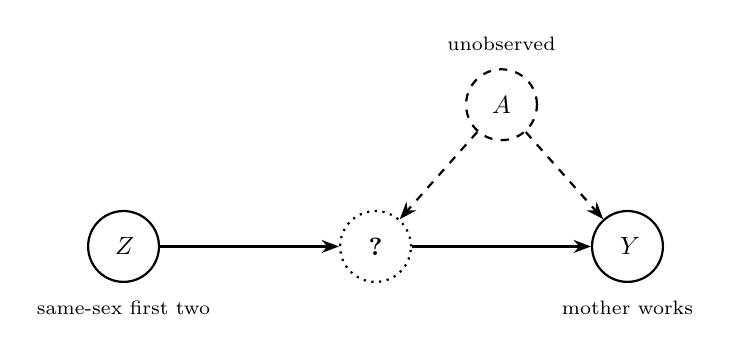
\begin{tikzpicture}[node distance=22mm]
\node[dnode] (Z) at (0,0) {$Z$};
\node[qnode] (Q) at (3.2,0) {\textbf{?}};
\node[dnode] (Y) at (6.4,0) {$Y$};
\node[unode] (A) at (4.8,1.8) {$A$};
\draw[de] (Z) -- (Q);
\draw[de] (Q) -- (Y);
\draw[dde] (A) -- (Q);
\draw[dde] (A) -- (Y);
\node[below=1mm of Z, font=\scriptsize] {same-sex first two};
\node[below=1mm of Y, font=\scriptsize] {mother works};
\node[above=1mm of A, font=\scriptsize] {unobserved};
\end{tikzpicture}
\end{center}

\begin{itemize}
\tightlist
\item
  You know the IV, the outcome, and maybe the confounders. \textbf{You
  do not know the treatment} --- and that missing link is the source of
  the strangeness.
\item
  Fill the hole with \textbf{family size}: parents who want a mix of
  sexes and get two of a kind try for a third child, and a third child
  changes labour supply.
\item
  Sex ratios are valid IVs for family size \emph{because} they move
  family size and are otherwise unrelated to the mother's labour supply.
\end{itemize}
\end{frame}

\begin{frame}{The strangeness principle}
\protect\phantomsection\label{the-strangeness-principle-1}
\begin{quote}
A valid IV neither directly causes the outcome, nor is correlated with
anything else that does --- \textbf{except through the treatment.}
\end{quote}

\begin{itemize}
\tightlist
\item
  In a valid DAG the only route from \(Z\) to \(Y\) runs \emph{through}
  \(D\).
\item
  Now look at the raw \(Z\)--\(Y\) correlation, in which \(D\) never
  appears. You see a real association and \textbf{no visible reason for
  one}, because the only thing that could explain it has been left out
  of the picture. \emph{That} is the strangeness --- and it is a symptom
  of validity, not a defect.
\item
  If the \(Z\)--\(Y\) association looks perfectly natural on its face,
  that usually means \(Z\) reaches \(Y\) by some route \emph{other} than
  \(D\) --- which is the next slide.
\end{itemize}
\end{frame}

\begin{frame}{When nothing feels strange, be suspicious}
\protect\phantomsection\label{when-nothing-feels-strange-be-suspicious}
\begin{center}
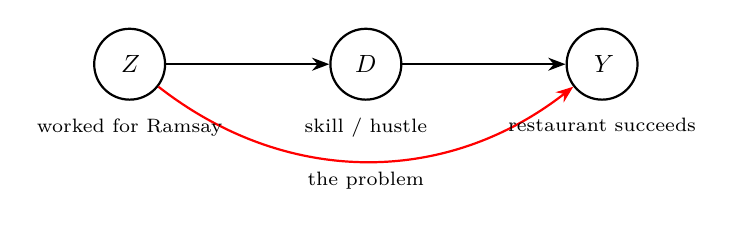
\begin{tikzpicture}[node distance=20mm]
\node[dnode] (Z) at (0,0) {$Z$};
\node[dnode] (D) at (3.0,0) {$D$};
\node[dnode] (Y) at (6.0,0) {$Y$};
\draw[de] (Z) -- (D);
\draw[de] (D) -- (Y);
\draw[de,red,thick] (Z) to[bend right=38] node[below,font=\scriptsize,midway,black] {the problem} (Y);
\node[below=1mm of Z, font=\scriptsize] {worked for Ramsay};
\node[below=1mm of D, font=\scriptsize] {skill / hustle};
\node[below=1mm of Y, font=\scriptsize] {restaurant succeeds};
\end{tikzpicture}
\end{center}

\begin{itemize}
\tightlist
\item
  Cousin Jacob became a chef. He was a line cook on one of Gordon
  Ramsay's shows, and credits his own hustle for everything since.
\item
  The table laughs. There is \textbf{nothing strange} about someone who
  worked with Ramsay going on to succeed --- his name alone brings
  investors, press, partnerships and early customers.
\item
  That red arrow is a direct path from IV to outcome. It is a violation
  of the \textbf{exclusion restriction}, and it cannot be fixed by any
  estimator.
\end{itemize}
\end{frame}

\begin{frame}{IVs are treatment assignment mechanisms}
\protect\phantomsection\label{ivs-are-treatment-assignment-mechanisms}
\begin{itemize}
\tightlist
\item
  \textbf{A valid IV corresponds to something in the real world that
  literally moves units into and out of treatment.} Coin flips. Draft
  numbers. Lotteries.
\item
  The best IVs come from \textbf{institutional knowledge} of how the
  treatment is actually assigned.
\item
  Talk to people. Ask them, in their own words, how some ended up
  treated and others did not.
\item
  You will notice this is the same discipline that §6.4 demanded of RD:
  \emph{know the rule}. Here: \emph{know the shock}.
\end{itemize}
\end{frame}

\section{7.2 The Wald Estimator}\label{the-wald-estimator}

\begin{frame}{When OLS is biased}
\protect\phantomsection\label{when-ols-is-biased}
\begin{center}
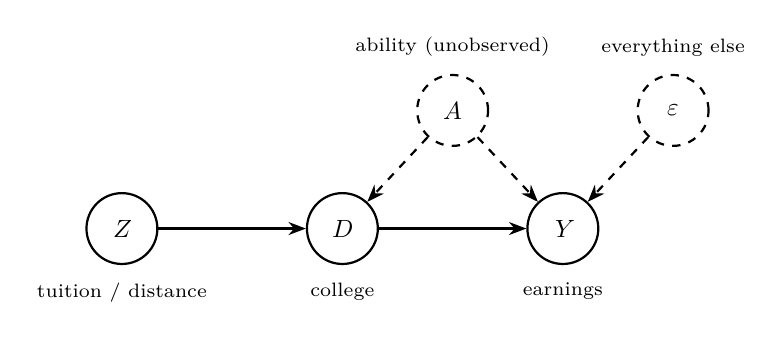
\begin{tikzpicture}[node distance=20mm]
\node[dnode] (Z) at (0,0) {$Z$};
\node[dnode] (D) at (2.8,0) {$D$};
\node[dnode] (Y) at (5.6,0) {$Y$};
\node[unode] (A) at (4.2,1.5) {$A$};
\node[unode] (E) at (7.0,1.5) {$\varepsilon$};
\draw[de] (Z) -- (D);
\draw[de] (D) -- (Y);
\draw[dde] (A) -- (D);
\draw[dde] (A) -- (Y);
\draw[dde] (E) -- (Y);
\node[below=1mm of Z, font=\scriptsize] {tuition / distance};
\node[below=1mm of D, font=\scriptsize] {college};
\node[below=1mm of Y, font=\scriptsize] {earnings};
\node[above=1mm of A, font=\scriptsize] {ability (unobserved)};
\node[above=1mm of E, font=\scriptsize] {everything else};
\end{tikzpicture}
\end{center}

\vspace{-0.5em}

Suppose the true model of earnings is \[
Y_i = \alpha + \delta D_i + \gamma A_i + \varepsilon_i,
\] but \(A\) is not in your data, so you estimate
\(Y_i = \alpha + \delta D_i + \eta_i\) with
\(\eta_i = \gamma A_i + \varepsilon_i\).

\begin{itemize}
\tightlist
\item
  \textbf{\(A\) and \(\varepsilon\) are both unobserved}, but they
  differ in one decisive way: \(A\) shifts who goes to college, while
  everything else, \(\varepsilon\), does not. Hence \(C(D,A) \neq 0\)
  but \(C(D,\varepsilon) = 0\).
\end{itemize}
\end{frame}

\begin{frame}{The omitted variable bias formula}
\protect\phantomsection\label{the-omitted-variable-bias-formula}
Write \(C(\cdot,\cdot)\) for covariance and \(V(\cdot)\) for variance.
OLS is a scaled covariance: \[
\hat\delta = \frac{C(Y, D)}{V(D)}.
\] Substitute the \emph{long} model for \(Y\) and expand: \[
\begin{aligned}
\hat\delta
&= \frac{\delta V(D) + \gamma\,C(D,A) + C(D,\varepsilon)}{V(D)} \\[0.3em]
&= \delta \;+\; \gamma\,\frac{C(A,D)}{V(D)}
\qquad\text{since } C(D,\varepsilon) = 0 .
\end{aligned}
\]
\end{frame}

\begin{frame}{The trick: take the covariance with \(Z\) instead}
\protect\phantomsection\label{the-trick-take-the-covariance-with-z-instead}
Keep the long model and compute \(C(Y,Z)\) rather than \(C(Y,D)\): \[
C(Y,Z) \;=\; \delta\,C(D,Z) \;+\; \gamma\,C(A,Z) \;+\; C(\varepsilon,Z).
\]

\begin{itemize}
\tightlist
\item
  If the DAG is true, \(C(A,Z) = 0\) and \(C(\varepsilon, Z) = 0\). \[
  C(Y,Z) = \delta\,C(D,Z).
  \]
\item
  Divide both sides by \(C(D,Z)\): \[
  \boxed{\;\hat\delta_{\text{Wald}} \;=\; \frac{C(Y,Z)}{C(D,Z)} \;=\; \delta\;}
  \]
\item
  This ratio is the Wald estimator, named after Abraham Wald (Wald
  1940).
\end{itemize}
\end{frame}

\begin{frame}{What makes it work, and what cannot be checked}
\protect\phantomsection\label{what-makes-it-work-and-what-cannot-be-checked}
The Wald estimator recovers \(\delta\) when:

\begin{enumerate}
\tightlist
\item
  \textbf{Exclusion.} \(Z\) does not cause \(Y\) directly --- any effect
  runs through \(D\). Equivalently, \(Z\) is \emph{excluded from} the
  \(Y\) equation: write it in and its coefficient is zero. Hence the
  standard phrase \textbf{``excluded instrument''}.
\item
  \textbf{Independence.} \(Z\) is independent of the confounder \(A\)
  and the error \(\varepsilon\).
\item
  \textbf{A nonzero first stage.} \(C(D,Z) \neq 0\).
\end{enumerate}

\vspace{0.4em}

\begin{itemize}
\tightlist
\item
  Under these, \(\operatorname{plim} \hat\delta = \delta\):
  \textbf{consistency}. In finite samples it differs, and by how much
  depends largely on the strength of that denominator --- §7.4.
\item
  Exclusion cannot be tested. Arguments for it are \emph{narrative}.
\item
  Good narratives rest on a realistic understanding of how treatment is
  actually assigned.
\item
  Defeating an IV paper requires only creating doubt about exclusion.
\end{itemize}
\end{frame}

\begin{frame}{Reduced form and first stage}
\protect\phantomsection\label{reduced-form-and-first-stage}
\[
\underbrace{\frac{C(Y,Z)}{C(D,Z)}}_{\textstyle \hat\delta_{\text{Wald}}}
\qquad=\qquad
\frac{\text{\textbf{Reduced form}}}{\text{\textbf{First stage}}}
\]

\begin{itemize}
\tightlist
\item
  The \textbf{reduced form}, \(C(Y,Z)\), is the strange association
  itself --- the \(Z\)--\(Y\) correlation that should not be there.
\item
  The \textbf{first stage}, \(C(D,Z)\), is the association between IV
  and treatment. It is what \emph{resolves} the strangeness.
\end{itemize}
\end{frame}

\section{7.3 Two Stage Least Squares}\label{two-stage-least-squares}

\begin{frame}{Wald \emph{is} 2SLS}
\protect\phantomsection\label{wald-is-2sls}
Start from the Wald ratio and multiply through by \(V(Z)/V(Z)\): \[
\hat\delta_{\text{Wald}}
= \frac{C(Y,Z)}{C(D,Z)}
= \frac{C(Y,Z)/V(Z)}{C(D,Z)/V(Z)}
= \frac{\hat\pi_1\,C(Y,Z)}{\hat\pi_1^{2}\, V(Z)}
= \frac{C(Y, \hat\pi_1 Z)}{V(\hat\pi_1 Z)},
\] where \(\hat\pi_1 = C(D, Z)/V(Z)\) is the first-stage slope from
\(D = \pi_0 + \pi_1 Z + \nu\).

\begin{itemize}
\tightlist
\item
  But \(\hat\pi_1 Z\) is, up to the constant, the \textbf{fitted value}
  \(\hat D\) from that first stage. So \[
  \hat\delta_{2SLS} = \frac{C(\hat D, Y)}{V(\hat D)} .
  \]
\item
  We are no longer using \(D\). We are using the part of \(D\) that the
  IV explains --- the part that is, by assumption, unrelated to \(A\).
\item
  \textbf{Without covariates, Wald and 2SLS are identical.}
\end{itemize}
\end{frame}

\begin{frame}[fragile]{Four ways, one number}
\protect\phantomsection\label{four-ways-one-number}
\begin{Shaded}
\begin{Highlighting}[]
\FunctionTok{suppressMessages}\NormalTok{(\{}\FunctionTok{library}\NormalTok{(haven); }\FunctionTok{library}\NormalTok{(AER)\})}
\NormalTok{card }\OtherTok{\textless{}{-}} \FunctionTok{as.data.frame}\NormalTok{(}\FunctionTok{read\_dta}\NormalTok{(}\StringTok{"data/card.dta"}\NormalTok{))}
\NormalTok{d }\OtherTok{\textless{}{-}}\NormalTok{ card[}\SpecialCharTok{!}\FunctionTok{is.na}\NormalTok{(card}\SpecialCharTok{$}\NormalTok{lwage) }\SpecialCharTok{\&} \SpecialCharTok{!}\FunctionTok{is.na}\NormalTok{(card}\SpecialCharTok{$}\NormalTok{educ) }\SpecialCharTok{\&} \SpecialCharTok{!}\FunctionTok{is.na}\NormalTok{(card}\SpecialCharTok{$}\NormalTok{nearc4), ]}

\NormalTok{w1 }\OtherTok{\textless{}{-}} \FunctionTok{cov}\NormalTok{(d}\SpecialCharTok{$}\NormalTok{lwage, d}\SpecialCharTok{$}\NormalTok{nearc4) }\SpecialCharTok{/} \FunctionTok{cov}\NormalTok{(d}\SpecialCharTok{$}\NormalTok{educ, d}\SpecialCharTok{$}\NormalTok{nearc4)        }\CommentTok{\# ratio of covariances}
\NormalTok{w2 }\OtherTok{\textless{}{-}} \FunctionTok{coef}\NormalTok{(}\FunctionTok{lm}\NormalTok{(lwage }\SpecialCharTok{\textasciitilde{}}\NormalTok{ nearc4, d))[}\DecValTok{2}\NormalTok{] }\SpecialCharTok{/} \FunctionTok{coef}\NormalTok{(}\FunctionTok{lm}\NormalTok{(educ }\SpecialCharTok{\textasciitilde{}}\NormalTok{ nearc4, d))[}\DecValTok{2}\NormalTok{]  }\CommentTok{\# ratio of OLS}
\NormalTok{fs }\OtherTok{\textless{}{-}} \FunctionTok{lm}\NormalTok{(educ }\SpecialCharTok{\textasciitilde{}}\NormalTok{ nearc4, d)}
\NormalTok{w3 }\OtherTok{\textless{}{-}} \FunctionTok{coef}\NormalTok{(}\FunctionTok{lm}\NormalTok{(d}\SpecialCharTok{$}\NormalTok{lwage }\SpecialCharTok{\textasciitilde{}} \FunctionTok{fitted}\NormalTok{(fs)))[}\DecValTok{2}\NormalTok{]                     }\CommentTok{\# manual two stages}
\NormalTok{w4 }\OtherTok{\textless{}{-}} \FunctionTok{coef}\NormalTok{(}\FunctionTok{ivreg}\NormalTok{(lwage }\SpecialCharTok{\textasciitilde{}}\NormalTok{ educ }\SpecialCharTok{|}\NormalTok{ nearc4, }\AttributeTok{data =}\NormalTok{ d))[}\DecValTok{2}\NormalTok{]       }\CommentTok{\# one command}
\FunctionTok{setNames}\NormalTok{(}\FunctionTok{unname}\NormalTok{(}\FunctionTok{c}\NormalTok{(w1, w2, w3, w4)),}
         \FunctionTok{c}\NormalTok{(}\StringTok{"covariances"}\NormalTok{, }\StringTok{"OLS ratio"}\NormalTok{, }\StringTok{"manual 2SLS"}\NormalTok{, }\StringTok{"ivreg"}\NormalTok{))}
\end{Highlighting}
\end{Shaded}

\begin{verbatim}
covariances   OLS ratio manual 2SLS       ivreg 
  0.1880626   0.1880626   0.1880626   0.1880626 
\end{verbatim}

\footnotesize

Card (1995), \(N = 3{,}010\). Compare OLS on the same data: 0.0521.
\end{frame}

\begin{frame}[fragile]{One warning about doing it by hand}
\protect\phantomsection\label{one-warning-about-doing-it-by-hand}
\begin{itemize}
\tightlist
\item
  Manual two-step 2SLS is fine to \textbf{see} the mechanics, never to
  \textbf{report}: second-stage SEs treat \(\hat D\) as data, so they
  are too small.
\item
  Use \texttt{ivreg} (R) or \texttt{ivregress\ 2sls} (Stata) for the
  correct variance.
\item
  More IVs than endogenous regressors means the model is
  \textbf{over-identified}, and 2SLS uses a weighted combination of the
  IVs. That is where §7.4's trouble begins.
\item
  Over-identification test (Sargan, or Hansen's \(J\) with robust SEs):
  do the IV-specific Wald estimates agree? A rejection is usually read
  as ``an IV is invalid''; §7.5 gives a second reason.
\end{itemize}
\end{frame}

\section{7.4 Weak Instruments}\label{weak-instruments}

\begin{frame}{Quarter of birth and compulsory schooling}
\protect\phantomsection\label{quarter-of-birth-and-compulsory-schooling}
\begin{itemize}
\tightlist
\item
  \textbf{Angrist and Krueger (1991).} Two institutional facts,
  combined:

  \begin{enumerate}
  \tightlist
  \item
    Children start first grade based on a \textbf{31 December} cutoff.
    Two children born a day apart, 31 December and 1 January, start a
    year apart --- purely by chance.
  \item
    Compulsory schooling laws let students leave at \textbf{16}.
  \end{enumerate}
\item
  A child born in the fourth quarter therefore reaches 16 having
  completed \emph{more} schooling than one born in the first quarter.
\item
  So quarter of birth shifts years of schooling --- a little, for some
  people --- and is otherwise, one hopes, unrelated to earnings.
\item
  \textbf{The strangeness test:} tell someone that people born in
  January earn less than people born in October. They will frown. Good.
\end{itemize}
\end{frame}

\begin{frame}{Present the Wald estimator as two pictures}
\protect\phantomsection\label{present-the-wald-estimator-as-two-pictures}
\begin{itemize}
\tightlist
\item
  Angrist and Krueger show the \textbf{first stage} --- years of
  schooling by quarter of birth, cohort by cohort --- as a figure.
  Fourth- and third-quarter births sit visibly higher.
\item
  They show the \textbf{reduced form} --- log weekly earnings by quarter
  of birth --- the same way. Jagged, but the 3s and 4s sit above the 1s
  and 2s.
\item
  Those two figures \emph{are} the numerator and the denominator of the
  Wald estimator.
\item
  \textbf{The rule for your own work:} visualise the reduced form and
  the first stage separately, even if you will ultimately report 2SLS. A
  plot of \(Y\) against \(\hat D\) is opaque and invites suspicion,
  because the data have already been processed.
\item
  A second thing the figure reveals: the relationship \textbf{fades for
  later cohorts}. By the 1947 births it has nearly vanished.
\end{itemize}
\end{frame}

\begin{frame}{A falsification test built into the first stage (Table
7.2)}
\protect\phantomsection\label{a-falsification-test-built-into-the-first-stage-table-7.2}
\begin{itemize}
\tightlist
\item
  Quarter of birth predicts \textbf{total schooling} and \textbf{high
  school graduation}, both negative and significant: born earlier in the
  year, less schooling. That is the first stage.
\item
  It does \textbf{not} predict \textbf{college graduation}. And that is
  the point.
\item
  Compulsory schooling binds only through high school. If quarter of
  birth predicted college completion, postgraduate degrees and total
  years alike, the IV would clearly be picking up something \emph{other}
  than the compulsory-schooling channel --- and exclusion would be in
  doubt.
\item
  \textbf{The general lesson.} Where your proposed mechanism implies the
  IV should have \emph{no} effect, show that it has no effect.
  Untestable assumptions have testable implications; go find them.
\end{itemize}
\end{frame}

\begin{frame}{More IVs, more precision --- at what price?}
\protect\phantomsection\label{more-ivs-more-precision-at-what-price}
\small

\begin{itemize}
\tightlist
\item
  Angrist and Krueger wanted more variation in predicted schooling,
  which should mean more precision. So they interacted the three quarter
  dummies with state and year of birth: \textbf{180 IVs}. It looked like
  a free lunch. It was not. Many extra IVs were \textbf{nearly useless}.
\item
  \textbf{Bound, Jaeger and Baker (1995)} showed what this does. Write
  both equations with their own errors,
  \(Y_i = \delta D_i + \varepsilon_i\) and \(D_i = Z_i'\pi + \nu_i\).
  Endogeneity \emph{is}
  \(\sigma_{\varepsilon\nu} \equiv C(\varepsilon_i,\nu_i) \neq 0\): the
  part of \(D\) the IVs cannot explain moves with the structural error.
  Then \[
  E[\hat\delta_{2SLS} - \delta] \;\approx\; \underbrace{\frac{\sigma_{\varepsilon\nu}}{\sigma_\nu^{2}}}_{\text{the OLS bias}} \cdot \frac{1}{F + 1},
  \] where \(F\) is the first-stage \(F\)-statistic.
\item
  As \(F \to \infty\) the bias vanishes; as \(F \to 0\) \textbf{2SLS
  converges on the OLS bias}. Adding weak instruments lowers \(F\) and
  so moves you back toward the thing you were trying to escape.
\end{itemize}
\end{frame}

\begin{frame}{How should we measure weakness?}
\protect\phantomsection\label{how-should-we-measure-weakness}
\begin{itemize}
\tightlist
\item
  \textbf{The old rule.} Stock and Yogo (2005): first-stage \(F > 10\).
  Based on Monte Carlo under homoskedasticity. For twenty years this was
  the standard.
\item
  \textbf{The number 10 is now considered too low}, especially with
  multiple endogenous regressors, heteroskedasticity, or non-normal
  errors. Lee et al.~(2022) argue the relevant threshold can be above
  \textbf{100}.
\item
  Weak instruments do not merely bias point estimates. They
  \textbf{distort inference}: standard errors come out too small and
  \(t\)-tests mislead.
\item
  \textbf{What to report now}, following Andrews, Stock and Sun (2019):

  \begin{enumerate}
  \tightlist
  \item
    The \textbf{effective \(F\)-statistic} of Montiel Olea and Pflueger
    (2013), which accounts for heteroskedasticity. In the
    just-identified case it reduces to the robust first-stage \(F\).
  \item
    \textbf{Anderson--Rubin confidence intervals} --- \emph{regardless}
    of the value of \(F\).
  \end{enumerate}
\end{itemize}
\end{frame}

\begin{frame}{Anderson--Rubin intervals}
\protect\phantomsection\label{andersonrubin-intervals}
\begin{itemize}
\tightlist
\item
  A conventional 2SLS interval is built \textbf{around a point
  estimate}: \(\hat\delta \pm 1.96\,\widehat{SE}(\hat{\delta})\). It
  presumes \(\hat\delta\) is well behaved, which under weak instruments
  it is not.
\item
  An AR interval instead \textbf{inverts a hypothesis test}. For each
  candidate value \(\delta_0\), it asks: could this value plausibly have
  generated the data? Values that could not are excluded.
\item
  AR intervals are valid \textbf{whether or not the IV is strong}.

  \begin{itemize}
  \tightlist
  \item
    Strong IV \(\Rightarrow\) the interval is tight.
  \item
    Weak instrument \(\Rightarrow\) the interval expands, sometimes to
    include both large positive and large negative values.
  \end{itemize}
\end{itemize}
\end{frame}

\begin{frame}{So what do you do with a weak instrument?}
\protect\phantomsection\label{so-what-do-you-do-with-a-weak-instrument}
\begin{itemize}
\tightlist
\item
  \textbf{Use a just-identified model with your single strongest IV.}
  Fewer, stronger beats more, weaker --- the opposite of the 1991
  intuition.
\item
  \textbf{Report AR intervals} and an effective \(F\). Let the reader
  see the weakness rather than discover it.
\item
  If you have a weak instrument problem, the only real solutions are to
  get a stronger IV or to stop doing IV. You are probably better off
  attacking the question another way.
\end{itemize}
\end{frame}

\section{7.5 Local Average Treatment
Effects}\label{local-average-treatment-effects}

\begin{frame}{Heckman's objection}
\protect\phantomsection\label{heckmans-objection}
\begin{itemize}
\tightlist
\item
  Everything so far assumed \textbf{homogeneous} treatment effects: one
  \(\delta\), the same for everyone. Drop that and the picture changes
  completely.
\item
  \textbf{Heckman (1990)} showed that IV identifies an average causal
  effect only under very strong conditions, later called
  \textbf{identification at infinity}: the IV would have to shift
  essentially the \emph{entire} population into or out of treatment.
\item
  Real IVs do nothing of the sort. The draft lottery did not compel
  service for everyone with a low number, nor exempt everyone with a
  high one.
\item
  So Heckman's critique appeared to undercut the most natural reading of
  Angrist's results.
\item
  And yet: the US government was literally randomising young men into
  the military. How could that reveal \emph{nothing} causal?
\item
  \textbf{Imbens and Angrist (1994)} worked backwards from that tension.
  If IVs cannot shift everyone, what exactly do they identify?
\end{itemize}
\end{frame}

\begin{frame}{Potential treatment status}
\protect\phantomsection\label{potential-treatment-status}
The move is to apply potential outcomes to the \textbf{first stage} as
well as the second: \[
D_i^{1} = i\text{'s treatment status when } Z_i = 1,
\qquad
D_i^{0} = i\text{'s treatment status when } Z_i = 0 .
\]

\begin{itemize}
\tightlist
\item
  Person \(i\) has \textbf{two hypothetical treatment statuses}, one for
  each value of the IV --- only one of which is ever realised.
\item
  The switching equation now applies to treatment: \[
  D_i = D_i^{0} + \underbrace{(D_i^{1} - D_i^{0})}_{\pi_{1i}} Z_i ,
  \] where \(\pi_{1i}\) is the \textbf{heterogeneous causal effect of
  the IV on treatment}.
\end{itemize}
\end{frame}

\begin{frame}{The five assumptions}
\protect\phantomsection\label{the-five-assumptions}
\small

\begin{enumerate}
\tightlist
\item
  \textbf{SUTVA} --- no spillovers, in the treatment \emph{or} in the
  IV.
\item
  \textbf{Independence} --- the IV is as good as randomly assigned.
\item
  \textbf{Exclusion} --- the IV reaches \(Y\) only through \(D\).
\item
  \textbf{Nonzero first stage} --- the IV actually moves \(D\).
\item
  \textbf{Monotonicity} --- it moves everyone the same way, or not at
  all.
\end{enumerate}

\vspace{0.5em}

\begin{itemize}
\tightlist
\item
  Compare RD, which rests on one assumption. This is why IV papers spend
  most of their length on assumptions rather than estimates.
\end{itemize}
\end{frame}

\begin{frame}{Assumption 1: SUTVA}
\protect\phantomsection\label{assumption-1-sutva}
\textbf{Person \(i\)'s potential treatment status and potential outcomes
depend only on \emph{their own} IV value and \emph{their own} treatment
--- not on anyone else's.}

\begin{itemize}
\tightlist
\item
  Potential outcomes always required this. What is new is that it now
  applies to the \textbf{first stage} too: \(D^1_i\) and \(D^0_i\) must
  be well defined for \(i\) whatever numbers everyone else draws.
\item
  \textbf{Violation through the IV.} I had no intention of enlisting and
  was not drafted. My best friend was drafted, so I went with him. My
  \(D_i\) depends on \emph{his} \(Z_i\).
\item
  \textbf{Violation through the treatment.} Mass conscription thins the
  civilian labour force, so wages change even for men who never served.
  Then \(Y^0_i\) is not a fixed quantity --- it depends on how many
  others were treated.
\item
  Peer effects, market-clearing prices and congestion are the usual
  suspects.
\end{itemize}
\end{frame}

\begin{frame}{Assumption 2: Independence}
\protect\phantomsection\label{assumption-2-independence}
\[\{\,Y_i(D^1_i,1),\; Y_i(D^0_i,0),\; D^1_i,\; D^0_i\,\} \indep Z_i\]

\begin{itemize}
\tightlist
\item
  ``As good as randomly assigned'': the IV is independent of potential
  outcomes \textbf{and} of potential treatment status. A draft number
  was drawn like a bingo ball --- it knew nothing about who you were.
\item
  \textbf{What it buys, first:} the reduced form becomes causal,
  \[E[Y_i \mid Z_i = 1] - E[Y_i \mid Z_i = 0] = E[Y_i(D^1_i,1)] - E[Y_i(D^0_i,0)].\]
\item
  \textbf{Second:} the first stage becomes causal,
  \[E[D_i \mid Z_i = 1] - E[D_i \mid Z_i = 0] = E[D^1_i - D^0_i].\]
\end{itemize}
\end{frame}

\begin{frame}{Assumption 3: Exclusion}
\protect\phantomsection\label{assumption-3-exclusion}
\[Y_i(D_i, 0) = Y_i(D_i, 1) \qquad \text{for } D_i = 0, 1\]

\begin{itemize}
\tightlist
\item
  Any effect of \(Z\) on \(Y\) must travel \textbf{through \(D\)}.
\item
  \textbf{The Vietnam violation.} A low lottery number pushed some men
  into service --- and pushed others into graduate school for a
  deferment. Schooling affects earnings directly, so the lottery reaches
  earnings by two routes, not one.
\item
  \textbf{Independence does not imply exclusion.} The lottery really was
  random, which secures independence. Exclusion is a separate claim
  about the \emph{channel} for causal effects of the IV.
\end{itemize}
\end{frame}

\begin{frame}{Assumption 4: Nonzero first stage}
\protect\phantomsection\label{assumption-4-nonzero-first-stage}
\[E[D^1_i - D^0_i] \neq 0\]

\begin{itemize}
\tightlist
\item
  The IV must actually move the average probability of treatment. Did a
  low lottery number raise the chance of serving? If so, the first stage
  holds.
\item
  It is the \textbf{denominator} of the Wald ratio. At zero the estimand
  does not exist; near zero it is unstable --- which was the whole of
  §7.4.
\item
  \textbf{The one testable assumption}: it involves \(D\) and \(Z\)
  only, and you have data on both. Report the first-stage coefficient,
  its robust SE, and the effective \(F\).
\item
  Note what is \emph{not} required: the IV need not move everyone, only
  a nonzero fraction. That concession is exactly what will make the
  estimand \textbf{local}.
\end{itemize}
\end{frame}

\begin{frame}{Assumption 5: Monotonicity}
\protect\phantomsection\label{assumption-5-monotonicity}
Recall the switching equation for the first stage,
\(D_i = D_i^{0} + \pi_{1i} Z_i\), so that
\[\underbrace{\pi_{1i} = D^1_i - D^0_i}_{i\text{'s own causal effect of } Z \text{ on } D}
\qquad\Longrightarrow\qquad
\text{either } \pi_{1i} \geq 0 \text{ for all } i, \ \text{ or } \pi_{1i} \leq 0 \text{ for all } i .\]

\begin{itemize}
\tightlist
\item
  The IV may leave some people untouched, but everyone it does move must
  move in the \textbf{same direction}. Draft eligibility pushes men into
  service or leaves them alone --- never out.
\item
  Equivalently: \textbf{no defiers.} Nobody serves \emph{only because}
  their number was \emph{not} called.
\item
  Without it, compliers' and defiers' effects enter the Wald ratio with
  opposite signs and can cancel. The estimand need not be a weighted
  average of the underlying individual causal effects.
\end{itemize}
\end{frame}

\begin{frame}{The LATE theorem}
\protect\phantomsection\label{the-late-theorem}
If all five assumptions hold, IV identifies \[
\delta_{\text{LATE}}
= \frac{\text{effect of } Z \text{ on } Y}{\text{effect of } Z \text{ on } D}
= \frac{E[Y_i(D^1_i,1) - Y_i(D^0_i,0)]}{E[D^1_i - D^0_i]}
= E\big[\,Y^1_i - Y^0_i \;\big|\; D^1_i - D^0_i = 1\,\big].
\]

\begin{itemize}
\tightlist
\item
  The average is taken \textbf{only over compliers} --- the people whose
  treatment status the IV actually changed. That conditioning is what
  the word \emph{local} means.
\item
  Heckman was right that IV cannot deliver the ATE. Imbens and Angrist's
  answer was not to argue with him, but to ask what IV \emph{does}
  deliver, and to name it.
\item
  \textbf{Angrist (1990) therefore estimated} the effect of military
  service on earnings \emph{for men who served because their number was
  called} --- which is arguably exactly the right policy parameter for a
  question about conscription.
\item
  Whether the complier group is the group you care about varies entirely
  by application. You must argue it, not assume it.
\end{itemize}
\end{frame}

\begin{frame}{Proof, and where each assumption enters}
\protect\phantomsection\label{proof-and-where-each-assumption-enters}
\footnotesize

A potential outcome has \emph{two} arguments, \(Y_i(d,z)\) --- four per
person. \textbf{Exclusion} says \(Y_i(d,1) = Y_i(d,0) \equiv Y^d_i\),
collapsing them to two: only now is \(\Delta_i \equiv Y^1_i - Y^0_i\)
well defined, and only now does \(Z\) reach \(Y\) through \(D\) alone.
(\textbf{SUTVA} makes them person-\(i\) quantities.) \[
Y_i = Y^0_i + \Delta_i D_i,
\quad
D_i = D^0_i + (D^1_i - D^0_i) Z_i
\;\Longrightarrow\;
Y_i = Y^0_i + \Delta_i \big[D^0_i + (D^1_i - D^0_i)Z_i\big].
\] \textbf{Independence} Evaluate that last line at \(Z_i = 1\) and at
\(Z_i = 0\): \[
Y_i\big|_{Z_i = 1} = Y^0_i + \Delta_i D^1_i,
\qquad
Y_i\big|_{Z_i = 0} = Y^0_i + \Delta_i D^0_i .
\] Independence leaves the distribution of
\((Y^0_i, \Delta_i, D^0_i, D^1_i)\) unchanged by \(Z_i\), so take
expectations and difference: \[
\underbrace{E[Y_i \mid Z_i{=}1] - E[Y_i \mid Z_i{=}0]}_{\text{reduced form}} = E\big[\Delta_i (D^1_i - D^0_i)\big],
\qquad
\underbrace{E[D_i \mid Z_i{=}1] - E[D_i \mid Z_i{=}0]}_{\text{first stage}} = E\big[D^1_i - D^0_i\big].
\] \textbf{Monotonicity} Now \(D^1_i - D^0_i \in \{0,1\}\): it is the
\textbf{complier indicator}, and an indicator inside an expectation is a
conditional mean times a probability: \[
E\big[\Delta_i(D^1_i - D^0_i)\big] = E[\Delta_i \mid C]\,P(C),
\qquad
E\big[D^1_i - D^0_i\big] = P(C), \qquad C \equiv \{D^1_i - D^0_i = 1\}.
\] \textbf{Nonzero first stage} \(P(C) > 0\), so divide. The \(P(C)\)
cancels: \(\ \delta_{\text{Wald}} = E[\Delta_i \mid C]\).
\(\qquad\blacksquare\)
\end{frame}

\begin{frame}{The four types}
\protect\phantomsection\label{the-four-types}
\begin{center}
\small
\begin{tabular}{llcc}
\toprule
Type & In the draft example & $D^0_i$ & $D^1_i$ \\
\midrule
\textbf{Compliers}    & serve if drafted, not otherwise        & $0$ & $1$ \\
Always-takers         & patriots: serve either way             & $1$ & $1$ \\
Never-takers          & conscientious objectors; medically exempt & $0$ & $0$ \\
\textit{Defiers}      & serve only if \emph{not} drafted        & $1$ & $0$ \\
\bottomrule
\end{tabular}
\end{center}

\begin{itemize}
\tightlist
\item
  \textbf{Only compliers contribute.} Always-takers and never-takers
  have \(D^1_i = D^0_i\), so they drop out of the numerator \emph{and}
  the denominator of the Wald ratio on their own --- no assumption
  required. Defiers are the only group that has to be assumed away.
\item
  Under homogeneous effects the partition is irrelevant, because
  compliers have the same effect as everyone else.
\end{itemize}
\end{frame}

\begin{frame}{If monotonicity fails}
\protect\phantomsection\label{if-monotonicity-fails}
\small

Recall \(\pi_{1i} = D^1_i - D^0_i\). Reduced form
\(= E[\Delta_i \pi_{1i}]\) and first stage \(= E[\pi_{1i}]\) as before.
But now \(\pi_{1i} \in \{-1,0,1\}\): \[
E[\Delta_i \pi_{1i}] = \underbrace{P(C)\,E[\Delta_i \mid C]}_{\pi_{1i} = 1} \;\underbrace{-\; P(F)\,E[\Delta_i \mid F]}_{\pi_{1i} = -1} \;+\; \underbrace{0}_{\pi_{1i} = 0},
\qquad
E[\pi_{1i}] = P(C) - P(F),
\]

\vspace{-0.6em}

\[
\delta_{\text{Wald}}
= \frac{P(C)\,E[\Delta_i \mid C] \;-\; P(F)\,E[\Delta_i \mid F]}{P(C) - P(F)} .
\]

\begin{itemize}
\tightlist
\item
  The weights still sum to one, but \textbf{one of them is negative.}
  That is not an average of anything: it can land outside the range of
  every individual effect.
\item
  \textbf{Example.} 50\% compliers with \(\Delta_i = 2\), 30\% defiers
  with \(\Delta_i = 6\). Then
  \(\delta_{\text{Wald}} = (1.0 - 1.8)/(0.5 - 0.3) = \mathbf{-4}\) --- a
  negative estimate where treatment helps \emph{everybody}.
\item
  \textbf{Homogeneous effects.} If \(\Delta_i = \delta\) for all \(i\)
  the numerator is \(\delta\,[P(C)-P(F)]\), so the ratio is \(\delta\)
  either way. Monotonicity is a price we pay for heterogeneity.
\item
  Defiers are unobservable, so monotonicity is argued, not tested.
\end{itemize}
\end{frame}

\begin{frame}{Compliers are defined by the IV}
\protect\phantomsection\label{compliers-are-defined-by-the-iv}
\small

\begin{itemize}
\tightlist
\item
  \textbf{Change the IV and you change the estimand.} Both IVs in this
  lecture target the \emph{same} treatment (years of schooling) and the
  \emph{same} outcome (log wages):
\end{itemize}

\begin{center}
\small
\begin{tabular}{lll}
\toprule
 & Angrist--Krueger (1991) & Card (1995) \\
\midrule
IV            & quarter of birth              & 4-year college in the county \\
Compliers     & teens who would quit at 16    & kids for whom living at home decided it \\
Margin priced & a year of \emph{high school}  & the \emph{college} years \\
2SLS          & $\approx 0.09$                & $0.188$ \\
\bottomrule
\end{tabular}
\end{center}

\begin{itemize}
\tightlist
\item
  The two IVs do not price the same \emph{year} of schooling, let alone
  for the same people. Neither is ``the'' return to education.
\item
  So ``one of you is wrong'' does not follow --- and the
  \textbf{over-identification test of §7.3 can reject for this reason
  alone.} Two valid IVs with different compliers \emph{should} disagree;
  rejection means ``not the same estimand'', not ``invalid IV''.
\item
  \textbf{Practical advice.} Report the complier share and their
  observable characteristics.
\end{itemize}
\end{frame}

\section{7.6 Card (1995): College in the
County}\label{card-1995-college-in-the-county}

\begin{frame}{The design}
\protect\phantomsection\label{the-design}
\[
Y_i = \alpha + \delta S_i + \gamma X_i + \varepsilon_i,
\]

\(Y\) log earnings, \(S\) years of schooling, and \(\varepsilon\)
containing \textbf{ability}. If ability raises both schooling and wages,
OLS is biased up.

\begin{itemize}
\tightlist
\item
  \textbf{The IV:} whether the respondent grew up in a county with a
  \textbf{four-year college}.
\item
  \textbf{Why it moves schooling:} proximity lowers the cost of
  attendance.
\item
  \textbf{Who are the compliers?} Not those who would always attend, nor
  those who never would. The compliers are people for whom the cost of
  leaving home is the binding constraint.
\item
  \textbf{The strangeness test:} why should the presence of a college in
  your childhood county affect your wages at 30? Only through schooling,
  one hopes. Is that believable?
\end{itemize}
\end{frame}

\begin{frame}[fragile]{The estimates}
\protect\phantomsection\label{the-estimates}
\begin{center}\small
\begin{tabular}{lc}
\toprule
 & Schooling \\
\midrule
Estimated effect of schooling & 0.188 \\
 & (0.026) \\
 & [0.144, 0.251] \\
\midrule
\multicolumn{2}{l}{\emph{First stage}} \\
College in the county instrument & 0.829 \\
 & (0.107) \\
Olea and Pflueger $F$-statistic & 60.374 \\
Obs & 3,010 \\
\bottomrule
\end{tabular}
\end{center}

\footnotesize

\begin{itemize}
\tightlist
\item
  Robust SEs in parentheses, \textbf{Anderson--Rubin} 95\% interval in
  brackets. Computed from \texttt{card.dta}, not copied --- this
  reproduces Remix Table 7.6.
\item
  Living in a college county buys \textbf{0.83 of a year} of schooling,
  and \(F \approx 60\) is comfortably strong.
\item
  \textbf{2SLS says 18.8\% per year of schooling. OLS on the same data
  says 5.2\%.} More than three times larger --- which is backwards, and
  is the next slide.
\end{itemize}
\end{frame}

\begin{frame}{Why is 2SLS \emph{larger} than OLS?}
\protect\phantomsection\label{why-is-2sls-larger-than-ols}
\begin{itemize}
\tightlist
\item
  If the problem were \textbf{ability bias}, OLS would be biased
  \emph{upward}, so 2SLS should come in \textbf{lower}.
\item
  \textbf{Measurement error?} Classical measurement error in schooling
  attenuates OLS toward zero, and IV repairs it. But people know their
  own years of schooling fairly well!
\item
  \textbf{Compliers genuinely have higher returns?} The compliers are
  people for whom the marginal cost of attending was the binding
  constraint. If they were \textbf{underinvesting} in education because
  of that constraint, the return to the schooling they were induced to
  get is high.
\item
  This is a case where LATE \(\neq\) ATE is the \emph{interesting}
  finding: it says something about liquidity constraints in education.
\item
  It is also unfalsifiable from the data alone. Treat it as an
  interpretation, and say so.
\end{itemize}
\end{frame}

\begin{frame}{Aside: classical measurement error attenuates OLS}
\protect\phantomsection\label{aside-classical-measurement-error-attenuates-ols}
We want \(Y_i = \alpha + \delta D^*_i + u_i\), but we observe
\(D_i = D^*_i + e_i\). \textbf{Classical} error means \(e_i\) is pure
noise: uncorrelated with \(D^*_i\) and with \(u_i\). Substitute
\(D^*_i = D_i - e_i\):
\[ Y_i = \alpha + \delta D_i + \underbrace{(u_i - \delta e_i)}_{\text{new error}},\qquad C(D_i,\; u_i - \delta e_i) = -\,\delta\,\sigma^2_e \neq 0.\]
\[\ \operatorname{plim} \hat\delta_{\text{OLS}} = \delta \cdot \lambda,\; \text{where}\; \lambda = \frac{\sigma^2_{D^*}}{(\sigma^2_{D^*} + \sigma^2_e)}\]

\begin{itemize}
\tightlist
\item
  \textbf{Attenuation:} the bias is toward zero.
\item
  Error in a \emph{control} variable is worse: it biases the
  coefficients on everything else, in no predictable direction.
\end{itemize}
\end{frame}

\begin{frame}{Aside: why IV repairs it}
\protect\phantomsection\label{aside-why-iv-repairs-it}
\(Z\) must be correlated with the \textbf{true} \(D^*\), and
uncorrelated with \(u\) \emph{and} with the measurement error \(e\).
Then the noise simply cancels: \[
\frac{C(Y,Z)}{C(D,Z)}
= \frac{\delta\,C(D^*,Z)}{C(D^* + e,\;Z)}
= \frac{\delta\,C(D^*,Z)}{C(D^*,Z)}
= \delta .
\]

\begin{itemize}
\tightlist
\item
  \textbf{So where do you find such a \(Z\)? Independent measurement of
  the same thing.} Each measure's error is its own, so each can
  instrument the other.
\item
  \textbf{Ashenfelter and Krueger (1994)}: they instrument a twin's
  \emph{self-reported} schooling with the \emph{sibling's} report of it,
  and the attenuation-corrected return comes out higher.
\item
  In finance: two data vendors' versions of the same variable, a
  restated figure against the original, a survey measure against an
  administrative one.
\end{itemize}
\end{frame}

\section{7.8 Presenting Your IV
Results}\label{presenting-your-iv-results}

\begin{frame}{Know your assignment mechanism}
\protect\phantomsection\label{know-your-assignment-mechanism}
\begin{itemize}
\tightlist
\item
  Spend the time. Call people. Ask them how units ended up treated. Be
  your own worst critic about why you think the IV is random and why you
  think exclusion holds.
\item
  \textbf{And be willing to lose.} If your IV is bad, finding that out
  early is a \emph{good} outcome --- a bad IV crowds out your time and
  creativity while taking you somewhere false.
\item
  The empirical crisis in 1970s labour economics came largely from
  assuming model conditions held rather than establishing that they did.
  That is the mistake to avoid.
\end{itemize}
\end{frame}

\begin{frame}{What an IV table must contain}
\protect\phantomsection\label{what-an-iv-table-must-contain}
\begin{enumerate}
\tightlist
\item
  \textbf{The OLS estimate}, so the reader can see what you are
  correcting and in which direction.
\item
  \textbf{The 2SLS estimate} with standard errors clustered
  appropriately.
\item
  \textbf{The first-stage coefficient on the excluded IV}, with its
  standard error --- usually in a bottom panel.
\item
  \textbf{The effective \(F\)-statistic} (Olea--Pflueger), not merely
  the classical one.
\item
  \textbf{Anderson--Rubin confidence intervals}, whatever the \(F\).
\item
  \textbf{The number of observations} and, where the design implies it,
  the complier share.
\end{enumerate}
\end{frame}

\begin{frame}{A checklist for an IV paper}
\protect\phantomsection\label{a-checklist-for-an-iv-paper}
\small

\begin{enumerate}
\tightlist
\item
  \textbf{Name the shock.} What physically moved units into treatment?
  Who was moved, who was not, and why was that not their choice?
\item
  \textbf{State the exclusion restriction in words}, as a sentence about
  the world, and then argue it. Expect to spend a page.
\item
  \textbf{Run the falsification tests your mechanism implies.} Where the
  IV should have no effect, show it has none --- Angrist and Krueger's
  college-graduation result is the template.
\item
  \textbf{Plot all three}: the IV, the first stage, the reduced form.
\item
  \textbf{Report the effective \(F\)} and \textbf{Anderson--Rubin
  intervals}. Prefer one strong IV to many weak ones.
\item
  \textbf{Describe the compliers} --- their share, their
  characteristics, and whether they are the population the question is
  about.
\item
  \textbf{Show the reduced form on its own.} If it is not there, no
  amount of scaling by a first stage will create it.
\item
  \textbf{Address monotonicity explicitly} if your IV is a
  decision-maker, a score, or anything with discretion behind it.
\item
  \textbf{State the estimand as a LATE}, and resist calling it ``the''
  effect.
\end{enumerate}
\end{frame}

\section{7.9 Concluding Remarks}\label{concluding-remarks}

\begin{frame}{What IV buys}
\protect\phantomsection\label{what-iv-buys}
\begin{itemize}
\tightlist
\item
  It is the design in this course that addresses \textbf{selection on
  unobservables} head-on. Matching conditions on what you measured; RD
  needs a rule; IV needs only a shock.
\item
  When the shock is real --- a lottery, a draft number, a randomly
  assigned judge --- the argument is as close to an experiment as
  observational data gets.
\item
  It reframes what you are looking for. The question stops being
  \emph{``what should I control for?''} and becomes \emph{``what, in the
  world, moved these units around?''} That is almost always the better
  question.
\end{itemize}
\end{frame}

\begin{frame}{What it costs}
\protect\phantomsection\label{what-it-costs}
\begin{itemize}
\tightlist
\item
  \textbf{Five assumptions, four of them untestable.} RD has one. This
  is the honest reason many applied researchers now avoid IV --- not
  that it fails to identify something, but that it is hard to imagine an
  IV satisfying all five.
\item
  \textbf{The estimand is a LATE} for a group you cannot name and did
  not choose. Its usefulness depends entirely on how close the
  compliers' effect is to everybody else's, which you cannot check.
\item
  \textbf{Weak instruments are worse than they look.}
\item
  \textbf{Exclusion is an argument, not a test.} That makes IV papers
  contestable in a way RD papers are not --- defeating a LATE requires
  only creating doubt.
\end{itemize}
\end{frame}

\begin{frame}{References}
\protect\phantomsection\label{references}
\tiny

\begin{itemize}
\tightlist
\item
  Andrews, I., J. Stock and L. Sun (2019). Weak Instruments in IV
  Regression: Theory and Practice. \emph{Annual Review of Economics} 11,
  727--753.
\item
  Angrist, J. (1990). Lifetime Earnings and the Vietnam Era Draft
  Lottery. \emph{AER} 80, 313--336.
\item
  Angrist, J. and W. Evans (1998). Children and Their Parents' Labor
  Supply. \emph{AER} 88, 450--477.
\item
  Angrist, J. and A. Krueger (1991). Does Compulsory School Attendance
  Affect Schooling and Earnings? \emph{QJE} 106, 979--1014.
\item
  Angrist, J. and A. Krueger (2001). Instrumental Variables and the
  Search for Identification. \emph{JEP} 15, 69--85.
\item
  Ashenfelter, O. and A. Krueger (1994). Estimates of the Economic
  Return to Schooling from a New Sample of Twins. \emph{AER} 84,
  1157--1173.
\item
  Bound, J., D. Jaeger and R. Baker (1995). Problems with Instrumental
  Variables Estimation. \emph{JASA} 90, 443--450.
\item
  Card, D. (1995). Using Geographic Variation in College Proximity to
  Estimate the Return to Schooling. In \emph{Aspects of Labour Market
  Behaviour}.
\item
  Cunningham, S. \emph{Causal Inference: The Remix}, Ch. 7 --- this
  lecture follows it closely.
\item
  Heckman, J. (1990). Varieties of Selection Bias. \emph{AER P\&P} 80,
  313--318.
\item
  Imbens, G. and J. Angrist (1994). Identification and Estimation of
  Local Average Treatment Effects. \emph{Econometrica} 62, 467--475.
\item
  Lee, D., J. McCrary, M. Moreira and J. Porter (2022). Valid
  \(t\)-ratio Inference for IV. \emph{AER} 112, 3260--3290.
\item
  Montiel Olea, J. and C. Pflueger (2013). A Robust Test for Weak
  Instruments. \emph{JBES} 31, 358--369.
\item
  Stock, J. and M. Yogo (2005). Testing for Weak Instruments in Linear
  IV Regression. In \emph{Identification and Inference for Econometric
  Models}.
\item
  Wald, A. (1940). The Fitting of Straight Lines if Both Variables Are
  Subject to Error. \emph{Annals of Mathematical Statistics} 11,
  284--300.
\end{itemize}
\end{frame}




\end{document}
